Il clustering, o analisi di raggruppamento, è una tecnica non supervisionata con lo scopo di aggregare i dati in \textit{cluster} o gruppi
tali che i dati all'interno di un gruppo siano più simili tra loro rispetto a quelli all'esterno\cite{liao2005clustering, zazzarro2009clustering}.

I metodi di clustering per elaborare dati statici di differenti tipologie sono cinque:

\begin{itemize}
  \item Metodi basati sul partizionamento.
  \item Metodi basati sulla gerarchia.
  \item Metodi basati sulla densità.
  \item Metdi basati su una griglia.
  \item Metodi basati sul modello.
\end{itemize}

Il clustering basato sul partizionamento si basa sull'idea di individuare \textit{k} punti e successivamente
eseguire l'assegnazione di ogni elemento del dataset a uno dei \textit{k} punti individuati nella prima fase.
In questo modo sono individuate \textit{k} partizioni, che corrispondono ad altrettanti cluster.
Questo metodo ha come vantaggio la semplicità e il ridotto numero di iperparametri,
è infatti necessario specificare a priori solo il valore di \textit{k}.
Due esempi di algoritmi~\cite{arora2016analysis} possono essere \textit{k-means} e \textit{k-medioid}:
entrambi partono dall'individuare \textit{k} punti a caso all'interno del dataset, successivamente eseguire l'assegnazione dei restanti elementi,
ricalcolare il centro del cluster in un caso, il medioide nell'altro e riperetere le operazioni fino a giungere a una convergenza ai centri dei cluster.
I limiti di questo approccio sono l'eccessiva rigidità delle regole applicate nella generazione dei cluster e la necessità di conoscere a prescindere il numero di cluster \textit{k}.

\begin{figure}
  \centering
  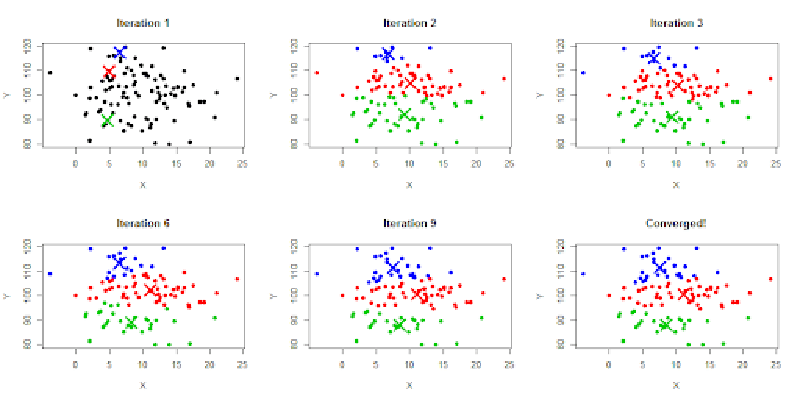
\includegraphics{/sec-1/KMeans.pdf}
  \caption{Fasi dell'algoritmo \textit{k-means},Fonte:~\url{http://www.learnbymarketing.com/methods/k-means-clustering/}}%
  \label{fig:chap-3:cute-overview}
\end{figure}



